\documentclass[a4paper,12pt]{article} % тип документа

% Поля страниц
\usepackage[left=2.5cm,right=2.5cm,
    top=2cm,bottom=2cm,bindingoffset=0cm]{geometry}
    
%Пакет дял таблиц   
\usepackage{multirow} 
    
%Отступ после заголовка    
\usepackage{indentfirst}


% Рисунки
\usepackage{floatrow,graphicx,calc}
\usepackage{wrapfig}

%%% Работа с картинками
\usepackage{graphicx}  % Для вставки рисунков
\graphicspath{{images/}{images2/}}  % папки с картинками
\setlength\fboxsep{3pt} % Отступ рамки \fbox{} от рисунка
\setlength\fboxrule{1pt} % Толщина линий рамки \fbox{}
\usepackage{wrapfig} % Обтекание рисунков и таблиц текстом

% Создаёем новый разделитель
\DeclareFloatSeparators{mysep}{\hspace{1cm}}

% Ссылки?
\usepackage{hyperref}
\usepackage[rgb]{xcolor}
\hypersetup{				% Гиперссылки
    colorlinks=true,       	% false: ссылки в рамках
	urlcolor=blue          % на URL
}


%  Русский язык
\usepackage[T2A]{fontenc}			% кодировка
\usepackage[utf8]{inputenc}			% кодировка исходного текста
\usepackage[english,russian]{babel}	% локализация и переносы




% Математика
\usepackage{amsmath,amsfonts,amssymb,amsthm,mathtools}

%%% Дополнительная работа с математикой
\usepackage{amsmath,amsfonts,amssymb,amsthm,mathtools} % AMS
\usepackage{icomma} % "Умная" запятая: $0,2$ --- число, $0, 2$ --- перечисление


% Что-то 
\usepackage{wasysym}


\begin{document}
\begin{center}
	\footnotesize{МОСКОВСКИЙ ФИЗИКО-ТЕХНИЧЕСКИЙ ИНСТИТУТ\\(НАЦИОНАЛЬНЫЙ 			ИССЛЕДОВАТЕЛЬСКИЙ УНИВЕРСИТЕТ)}\\
	\footnotesize{ФИЗТЕХ-ШКОЛА РАДИОТЕХНИКИ И КОМПЬЮТЕРНЫХ ТЕХНОЛОГИЙ\\}
	\hfill \break
	\hfill \break
	\hfill \break
	\hfill \break
	\hfill \break
	\hfill \break
\end{center}

\begin{center}   
    \hfill \break
	\hfill \break
	\hfill \break
	\hfill \break
	\hfill \break
	\hfill \break
	\hfill \break
	\hfill \break
	\hfill \break
	\hfill \break
	\hfill \break
	\large{Лабораторная работа № 3.1.3\\\large{\textbf{Измерение магнитного поля Земли}}}\\
	\hfill \break
	\hfill \break
	\hfill \break
	\hfill \break
	\hfill \break
	\hfill \break
	\hfill \break
	\hfill \break
	\hfill \break
	\hfill \break
	\hfill \break
	\begin{flushright}
		Климова Екатерина\\
		Группа Б01-108
	\end{flushright}
	\hfill \break
\end{center}
\hfill \break
\hfill \break
\begin{center}
	Долгопрудный, 2022 г.
\end{center}
\thispagestyle{empty}

\newpage
\hfill \break
\textbf{Цель работы:} исследовать свойства постоянных неодимовых магнитов; измерить с их помощью горизонтальную и вертикальную составляющие магнитного поля Земли и магнитное наклонение.
\hfill \break
\hfill \break
\textbf{В работе используются:} неодимовые магниты; тонкая нить для изготовления крутильного маятника; медная проволока; электронные весы; секундомер; измеритель магнитной индукции; штангенциркуль; брусок, линейка и штатив из немагнитных материалов; набор гирь и разновесов.

\section{Аннотация}
\hfill \break
В работе определяются вертикальная и горизонтальная составляющие магнитного поля Земли, а также магнитное наклонение. Сделать это предлагается при помощи совершающих крутильные колебания маятников, составленных из нескольких неодимовых магнитных шариков.

\section{Теоретические сведения}
\hfill \break
Простейший магнитный диполь может быть образован витком с током или постоянным магнитом. По определению, магнитный момент $\mathfrak{m}$ тонкого витка площадью $S$ с током $I$ равен (в системе СИ) 
$$
\mathfrak{m} = I\textbf{S},
$$
где $\textbf{S} = S\textbf{n}$ $-$ вектор площади контура, образующий с направлением тока правовинтовую систему, $\textbf{n}$ $-$ единичный вектор нормали к площадке. Если размеры контура с током или магнитной стрелки малы по сравнению с расстоянием до диполя, то соответствующий магнитный диполь называют \textit {элементарным}, или \textit {точечным}.

\hfill \break Магнитное поле точечного диполя определяется по формуле, аналогичной формуле для поля элементарного электрического диполя: 

$$
\textit{\textbf{B}}_\text{дип}=\frac{\mu_0}{4\pi}(\frac{3(\mathfrak{m}\cdot\textbf{\textit{r}})\textit{\textbf{r}}}{r^5}-\frac{\mathfrak{m}}{r^3}).
$$

\hfill \break Во внешнем магнитном поле с индукцией \textit{\textbf{B}} на точечный магнитный диполь $\mathfrak{m}$ действует механический момент сил 

$$
\mathfrak{M} = [\mathfrak{m} \times \textbf{\textit{B}}].
$$

\hfill \break При этом потенциальная энергия, которой обладает диполь с постоянным $\mathfrak{m}$, равна 

$$
W = -(\mathfrak{m} \cdot \textbf{\textit{B}}).
$$

\hfill \break Когда диполь ориентирован вдоль внешнего поля, то есть вектор его магнитного момента параллелен вектору магнитной индукции, он находится в состоянии \textit {равновесия} ($\textbf{\textit{M}} = 0$). При этом \textit {устойчивым} будет только состояние, в котором диполь сонаправлен с полем, поскольку так его потенциальная энергия достигает минимума.

\hfill \break В неоднородном магнитном поле на диполь, помимо момента сил, действует сила

$$
\textit{\textbf{F}} = (\mathfrak{m} \cdot \nabla)\textit{\textbf{B}}.
$$

\hfill \break Таким образом, \textit {свободный} магнитный диполь в неоднородном магнитном поле ориентируется вдоль силовых линий магнитного поля и втягивается в область более сильного поля, поскольку это ведет к уменьшению энергии диполя. 

\hfill \break Можно рассчитать силу взаимодействия двух магнитов с моментами $\mathfrak{m}_1$ и $\mathfrak{m}_2$ в рамках модели точечных диполей. В частном случае, когда моменты двух небольших магнитов направлены вдоль соединяющей их прямой: $\mathfrak{m}_\text{1, 2} || \textbf{\textit{r}},$ где $\textbf{\textit{r}}$ $-$ радиус-вектор между ними, магниты взаимодействуют с силой

$$
F_{12} = -\frac{6\mathfrak{m}_{1}\mathfrak{m}_{2}}{r^4}.
$$

\hfill \break Здесь магниты притягиваются, если их магнитные моменты сонаправлены, и отталкиваются, если направлены противоположно.

\hfill \break Если магнитные моменты направлены перпендикулярно соединяющей их прямой (радиус-вектору), то сила их взаимодействия окажется в два раза меньше и будет иметь противоположный знак:

$$
F_{12} = \frac{3\mathfrak{m}_{1}\mathfrak{m}_{2}}{r^4}
$$

\hfill \break (диполи отталкиваются, если их магнитные моменты сонаправлены, и притягиваются, если направлены противоположно).

\section{Экспериментальная установка}

 \hfill \break Для проведения эксперимента важно, что а) вещество, из которого изготовлены магниты, является \textit {магнитожестким} материалом; б) шары намагничены однородно. 

\hfill \break Магнитное поле однородного намагниченного шара радиусом $R$ может быть вычислено точно. На расстояниях $r \geq R$ от центра шара оно совпадает с полем \textit{точечного} магнитного диполя, расположенного в центре, магнитный момент $\mathfrak{m}$ которого совпадает с полным моментом шара. Внутри шара магнитное поле однородно. Hетрудно получить, что при $r < R$ \[\textbf{\textit{B}}_{0} = \frac{\mu_0 \mathfrak{m}}{2\pi R^3}\]

\hfill \break В качестве ещё одной характеристики материала магнита используют остаточную \textit {намагниченность} $\textbf{M}$. По определению, намагниченность равна \textit {объёмной плотности магнитного момента}, поэтому для однородного намагниченного шара $$\mathfrak{m}= \textbf{M}V ,$$ где $\displaystyle V = \frac{4\pi}{3}R^3$ $-$ объём магнита. Величину $\textbf{\textit{B}}_r = \mu_0 \textbf{M}$ называют остаточной индукцией материала.

\hfill \break Из сказанного выше нетрудно видеть, что индукция $\textbf{B}_p$ \textit{на полюсах} однородно намагниченного шара направлена по нормали к поверхности и совпадает поэтому с индукцией внутри шара $\textbf{\textit{B}}_p = \textbf{\textit{B}}_0$. Величина $B_p$ связана с остаточной индукцией $B_r$ соотношением \[B_p = B_o = \frac{2}{3}B_r \]


\subsection{Определение магнитного момента магнитных шариков}

\hfill \break \textbf{Метод А.} Величину магнитного момента $\mathfrak{m}$ двух одинаковых шариков можно рассчитать, зная их массу $m$ и определив максимальное расстояние $r_{max}$, на котором они ещё удерживают друг друга в поле тяжести. При максимальном расстоянии сила тяжести шариков $mg$ равна силе их магнитного притяжения. 

\begin{wrapfigure}{r}{0.3\textwidth}
\begin{center}
    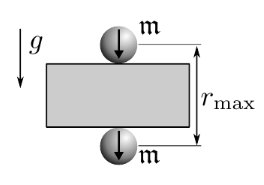
\includegraphics[width=1\textwidth]{3.1.3_1.png}
\end{center}
\end{wrapfigure}

\hfill \break Когда векторы двух магнитных моментов ориентированы вертикально, имеем

\begin{equation*}
    \mathfrak{m} = \sqrt{\frac{2\pi mgr^4_{max}}{3 \mu_0}} \
\end{equation*}

\hfill \break По величине $\mathfrak{m}$ можно рассчитать величину индукции $\textbf{\textit{B}}$ вблизи любой точки на поверхности шара радиуса $R$. Максимальная величина индукции наблюдается на полюсах.

\hfill \break \textbf{Метод Б.} Величину магнитного момента шариков можно определить также по силе их сцепления. Она определяется как сила, необходимая для разрыва двух сцепившихся магнитных шариков. Сила сцепления максимальна, если шары соединяются своими противоположными полюсами (магнитные моменты сонаправлены).

\begin{wrapfigure}{r}{0.3\textwidth}
\begin{center}
    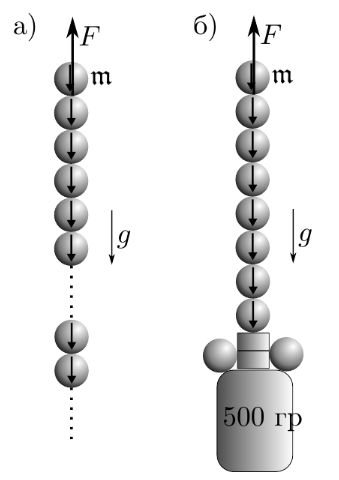
\includegraphics[width=1\textwidth]{3.1.3_2.png}
\end{center}
\end{wrapfigure}


\hfill \break Максимальную силу сцепления можно определить по весу магнитной цепочки, которую способен удержать самый верхний магнитный шарик. Если цепь состоит из одинаковых магнитных шариков, то при определённой длине она отрывается от верхнего шарика. При этом, учитывая, что сила притяжения убывает как $F \propto 1/r^4$, где $r$ — расстояние между центрами шаров, для расчёта прочности цепочки достаточно учитывать силу взаимодействия верхнего шара с 3–4 ближайшими соседями.

\hfill \break Сила сцепления двух одинаковых шаров с радиусами $R$ с магнитными моментами $\mathfrak{m}$ равна 

\begin{equation*}
        F_0 = \frac{3 \mu_0 \mathfrak{m}^2}{32 \pi R^4}\    
\end{equation*}

\hfill \break
Тогда минимальный вес цепочки, при котором она оторвётся от верхнего шарика, равен

\begin{equation*}
    F = F_0\left(1 + \frac{1}{2^4} + \frac{1}{3^4} + ... \right) \approx 1,08F_0.
\end{equation*}

\hfill \break
Отметим, что не обязательно составлять цепочку только из одинаковых шариков: на расстояниях, превышающих 20–30 диаметров шариков, можно подцепить любой груз, притягиваемый магнитом, на результат это не повлияет, в чём несложно убедиться экспериментально.

\subsection{Измерение горизонтальной составляющей индукции магнитного поля Земли}

\hfill \break Магнитная стрелка образована сцепленными друг с другом $n$ намагниченными шариками. С помощью $\Lambda$-образного подвеса стрелка подвешена в горизонтальном положении. Магнитные моменты всех шариков направлены в одну сторону вдоль оси стрелки. Под действием механического момента сил, действующего на стрелку со стороны поля Земли, стрелка стремится повернуться по горизонтальной составляющей магнитного поля Земли в направлении Юг$-$Север.

\begin{wrapfigure}{r}{0.3\textwidth}
\begin{center}
    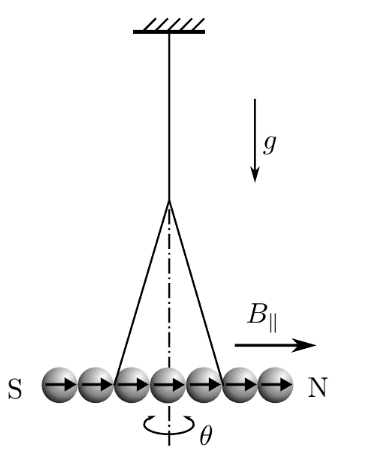
\includegraphics[width=1\textwidth]{3.1.3_3.png}
\end{center}
\end{wrapfigure}

\hfill \break При отклонении стрелки на малый угол $\theta$ ($\sin{\theta} \approx \theta$) от равновесного положения в горизонтальной плоскости возникают крутильные колебания вокруг вертикальной оси, проходящей через середину стрелки. Тогда уравнение крутильных колебаний:

$$
\mathfrak{M} = -\mathfrak{m}_{n}\textit{B}_{||}\sin{\theta}
$$

$$
J_{n}\ddot{\theta} + \mathfrak{m}_{n}B_{||}\theta = 0
$$

\hfill \break Отсюда находим период малых колебаний:

$$
T = 2\pi\sqrt{\frac{J_{n}}{\mathfrak{m}_{n}B_{||}}}.
$$

\hfill \break Момент инерции $J_{n}$ стрелки из $n$ шариков:

$$
J_{n} = \frac{1}{3}n^3mR^2.
$$

\hfill \break Тогда период колебаний маятника пропорционален числу шаров $n$, составляющих стрелку:

$$
T_{n} = 2\pi\sqrt{\frac{mR^2}{3\mathfrak{m}B_{||}}}\cdot n.
$$

\subsection{Измерение вертикальной составляющей индукции магнитного поля Земли. Магнитное наклонение}

\hfill \break В этом случае стрелка, составленная из четного числа одинаковых шаров и подвешенная за середину, расположится не горизонтально, а под некоторым углом к горизонту. Это связано с тем, что вектор индукции магнитного поля Земли не горизонтален, а образует с горизонтом некоторый угол $\beta,$ зависящий от географической широты $\phi$ места, где проводится опыт. Величина угла $\beta$ называется \textit {магнитным наклонением}.

\hfill \break \begin{center}
\begin{tabular}{cc}
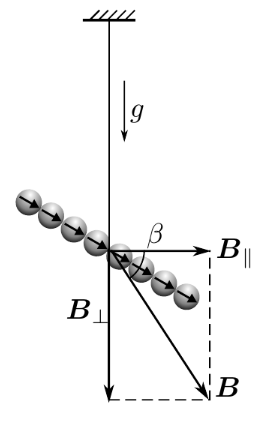
\includegraphics[width=0.2\textwidth]{3.1.3_4.png}&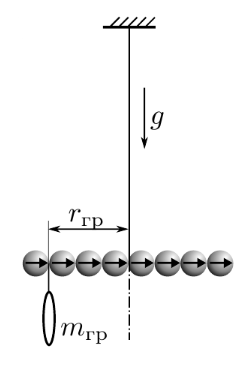
\includegraphics[width=0.2\textwidth]{3.1.3_5.png}\\
a)&б)\\
\end{tabular}
\end{center}

\hfill \break Избавиться от наклона можно, если выровнять стрелку горизонтально с помощью небольшого дополнительного грузика. В этом случае момент силы тяжести грузика относительно точки подвеса будет равен моменту сил, действующих на стрелку со стороны вертикальной составляющей магнитного поля Земли. Если масса груза равна $m_\text{гр}$, плечо силы тяжести $r_\text{гр}$, а полный магнитный момент стрелки $\mathfrak{m}_{n} = n\mathfrak{m}$, то в равновесии

$$
\mathfrak{M} = m_\text{гр}gr_\text{гр} = n\mathfrak{m}B_{\perp}.
$$

\section{Ход работы}

\subsection{Определение магнитного момента, намагниченности и остаточной магнитной индукции вещества магнитных шариков}

\hfill \break Для начала определим диаметр шарика при помощи штангенциркуля: $d = 0.6 \pm 0.001$ см, взвесим шарик: $m = 0.842  \pm 0.001$ г, с помощью магнетометра измерим индукцию поля на полюсах шарика: $B_{p1} = 231 \pm 0.5$ мТл. Для удобства занесем результаты подготовительных измерений в таблицу:

\begin{center}
\begin{tabular}{|c|c|c|}\hline
$d$, см&$m$, г&$B_{p1}$, мТл\\\hline
$0.6 \pm 0.001$&$0.842 \pm 0.001$&$231 \pm 0.5$\\\hline
\end{tabular}\\
\hfill \break \textbf {Таблица 1.} Подготовительные измерения~\\
\end{center}

\hfill \break Прокладывая бруски и листы бумаги между двумя шариками, определим максимальное расстояние $r_{max} = 1.78 \pm 0.05$ см, на котором шарики могут удерживать друг друга в поле тяжести Земли. Рассчитаем величину магнитного момента шарика: $\mathfrak{m}_{1} = \sqrt{\frac{mgr^4_{max}}{6}} = (3.7 \pm 0.2) \cdot 10^{-2}$ Дж/Тл. Погрешность можно рассчитать по формуле:

$$
\mathcal{E}_{\mathfrak{m}_{1}} = \sqrt{(\frac{\sigma{m}}{m})^2 + 4(\frac{\sigma{r_{max}}}{r_{max}})^2} \approx 6 \%.
$$

\hfill \break Теперь рассчитаем магнитный момент вторым способом $-$ при помощи цепочки из шариков. Минимальная масса составленной системы, при которой она отрывается от верхнего шарика, получилась равна $m_{min} = 212.4 \pm 1$ г. Тогда вес $F = m_{min}g = 1.08F_{0} = 1.08 \cdot \frac{3\mathfrak{m_{2}}^2}{8r^4}$, откуда $\mathfrak{m}_{2} = \sqrt{\frac{8F_{0}r^4}{3}} = \sqrt{\frac{8m_{min}gr^4}{1.08 \cdot 3}} = (6.5 \pm 0.1) \cdot 10^{-2}$ Дж/Тл. Погрешность рассчитывается по формуле:

$$
\mathcal{E}_{\mathfrak{m}_{2}} = \sqrt{(\frac{\sigma{m_{min}}}{m_{min}})^2 + 4(\frac{\sigma{r}}{r})^2} \approx 2 \%.
$$

\hfill \break Для определения наиболее точного метода измерения магнитного момента рассчитаем для каждого из них остаточную индукцию магнитного поля. Перед этим рассчитаем намагниченность (в единицах СГС):

$$
\textbf{\textit{M}}_1 = \frac{3\mathfrak{m}_{1}}{4\pi r^3} \approx 336 \pm 17;
$$

$$
\mathcal{E}_{\textbf{\textit{M}}_{1}} = \sqrt{(\frac{\sigma{\mathfrak{m}_{1}}}{\mathfrak{m}_{1}})^2 + 3(\frac{\sigma{r}}{r})^2} \approx 5 \%;
$$

$$
\textbf{\textit{M}}_2 = \frac{3\mathfrak{m}_{2}}{4\pi r^3} \approx 574 \pm 11;
$$

$$
\mathcal{E}_{\textbf{\textit{M}}_{2}} = \sqrt{(\frac{\sigma{\mathfrak{m}_{2}}}{\mathfrak{m}_{2}})^2 + 3(\frac{\sigma{r}}{r})^2} \approx 2 \%.
$$

\hfill \break Теперь рассчитаем остаточную индукцию (в единицах СГС): 

$$
\textbf{\textit{B}}_{r1} = 4\pi \textbf{\textit{M}}_1 = 4222 \pm 211;
$$

$$
\mathcal{E}_{\textbf{\textit{B}}_{r1}} = \mathcal{E}_{\textbf{\textit{M}}_{1}} \approx 5 \%;
$$

$$
\textbf{\textit{B}}_{r2} = 4\pi \textbf{\textit{M}}_2 = 7213 \pm 144;
$$

$$
\mathcal{E}_{\textbf{\textit{B}}_{r2}} = \mathcal{E}_{\textbf{\textit{M}}_{2}} \approx 2 \%.
$$

\hfill \break Табличное значение остаточной индукции для материала NdFeB $\textbf{\textit{B}}_{r} = 10 - 12$ ед. СГС, из чего можно сделать вывод, что второй способ измерения величины магнитного момента был более точным. Тем не менее, полученное в ходе эксперимента значение остаточной индукции достаточно сильно отличается от теоретического, что можно объяснить высокой неточностью измерений.

\subsection{Определение горизонтальной составляющей магнитного поля Земли}

\hfill \break Соберем крутильный маятник из 12 магнитных шариков и подвесим его на немагнитном штативе. Используя $\Lambda$-образный подвес, установим получившуюся магнитную стрелку в горизонтальное положение, а затем возбудим крутильные колебания маятника вокруг вертикальной оси и оценим их период. Исследуем зависимость периода крутильных колебаний от количества магнитных шариков, составляющих стрелку. Результаты занесем в таблицу и построим график зависимости $T(n)$:

\begin{center}
    \begin{tabular}{|c|c|c|c|c|}\hline
    $n_{\text{шар}}$ & $n_{\text{колеб}}$ & $t$, с & $T$, с & $\varepsilon_T$, \%\\ \hline
        11 & 6 &  23.6 & 3.93 & 2 \\ \hline
        9  & 6 &  19.7 & 3.28 & 2 \\ \hline
        8  & 8 &  23.3 & 2.91 & 2 \\ \hline
        7  & 9 &  22.7 & 2.52 & 2 \\ \hline
        6  & 8 &  17.1 & 2.13 & 2 \\ \hline
        5  & 8 &  14.2 & 1.78 & 2 \\ \hline
        4  & 10 & 14.4 & 1.44 & 2 \\ \hline
\end{tabular}\\
\hfill \break \textbf {Таблица 2.} Зависимость периода от количества шариков\\
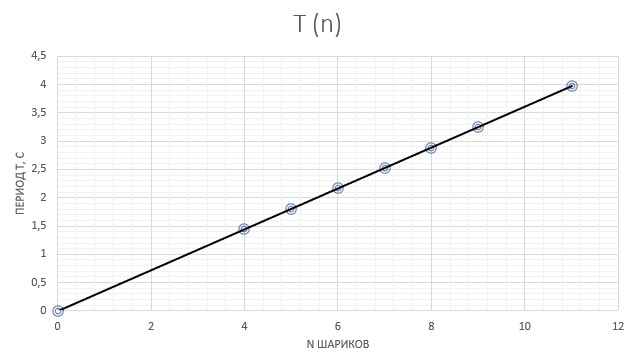
\includegraphics[width=0.95\textwidth]{3.1.3_6.png}\\
График зависимости $T$ $(n)$~\\
\end{center}

\hfill \break По углу наклона графика можно определить значение горизонтальной составляющей магнитного поля Земли $B_{||} = \frac{4\pi^{2}mr^2}{3\mathfrak{m}k^2} = (1.18 \pm 0.02) \cdot 10^{-5}$ Тл.

\subsection{Определение вертикальной составляющей магнитного поля Земли}

\hfill \break Изготовим магнитную стрелку из $n$ шариков и подвесим ее за середину с помощью нити на штативе. Определим момент сил, действующий со стороны магнитного поля Земли на горизонтально расположенную магнитную стрелку, для чего с помощью кусочков проволоки и грузов уравновесим стрелку в соответствующем положении. Проведем измерения момента сил для различных количеств шариков:

\begin{center}
    \begin{tabular}{|c|c|c|}\hline
    $n_{\text{шар}}$ & $\mathfrak{M}$, мкН$\cdot$м & $\varepsilon_M$, \% \\ \hline 
        12 & 418 & 5 \\ \hline
        10 & 314 & 5 \\ \hline
        8  & 209 & 5 \\ \hline
        6  & 191 & 5 \\ \hline
        4  & 150 & 5 \\ \hline
\end{tabular}\\
\hfill \break \textbf {Таблица 3.} Зависимость момента сил от количества шариков~\\
\end{center}

\hfill \break По полученным данным построим график зависимости $\mathfrak{M} (n)$:

\begin{center}
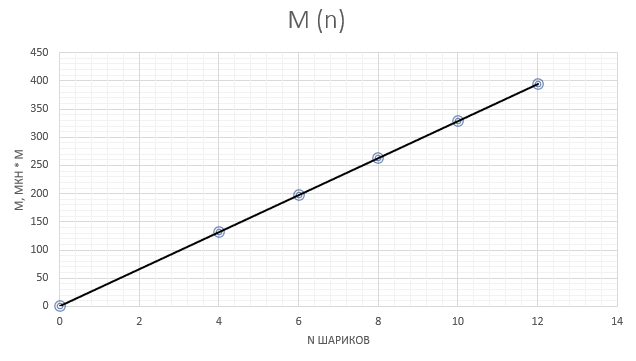
\includegraphics[width=0.95\linewidth]{3.1.3_7.png}\\
График зависимости $\mathfrak{M}$ $(n)$\\
\end{center}

\hfill \break Данные плохо легли на график, что может быть обусловлено тем, что набор возможных грузов дискретен, следовательно, момент сил не может быть подобран точно. По наклону прямой можно вычислить значение вертикальной составляющей магнитного поля Земли: $B_{\perp} = \frac{k}{\mathfrak{m}} = (3.30 \pm 0.44) \cdot 10^{-5}$ Тл. Теперь мы можем вычислить значение магнитного наклонения ($\tg{\beta} = \frac {B_{\perp}}{B_{||}}$, откуда $\beta \approx 70.32^{\circ}$, в то время как теоретическое значение $-$ примерно $72^{\circ}$) и суммарное магнитное поле Земли: $B = \sqrt{B_{\perp}^2 + B_{||}^2} = (3.5 \pm 0.44) \cdot 10^{-5}$ Тл. При этом табличное значение магнитного поля Земли в Московском регионе $-$ примерно $5 \cdot 10^{-5}$ Тл.

\section{Вывод}

\hfill \break В данной работе были экспериментально определены значения магнитного поля Земли и магнитного наклонения при помощи магнитных шариков, составлявших магнитную стрелку. Итоговые значения получились достаточно близки к табличным.

\end{document}
